\resizebox{0.7\columnwidth}{!}{
	\centering




	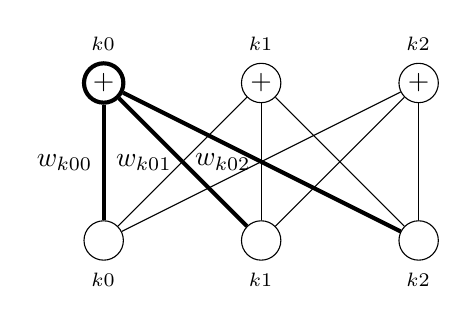
\begin{tikzpicture}[node distance=2cm, auto]

		% Upper layer nodes with increased size
		\node[draw, circle, minimum size=0.5cm,inner sep=1pt, line width=1.5pt] (A1) at (0, 2) {$+$};
		\node[draw, circle, minimum size=0.5cm,inner sep=1pt] (A2) at (2, 2) {$+$};
		\node[draw, circle, minimum size=0.5cm,inner sep=1pt] (A3) at (4, 2) {$+$};
		% Lower layer nodes with increase size
		\node[draw, circle, minimum size=0.5cm] (B1) at (0, 0) {};
		\node[draw, circle, minimum size=0.5cm] (B2) at (2, 0) {};
		\node[draw, circle, minimum size=0.5cm] (B3) at (4, 0) {};

		% Labels for the upper layer
		\node at (0, 2.5) {$\Qcircuit_{k0}$};
		\node at (2, 2.5) {$\Qcircuit_{k1}$};
		\node at (4, 2.5) {$\Qcircuit_{k2}$};

		% Labels for the lower layer
		\node at (0, -0.5) {$\tildeQcircuit_{k0}$};
		\node at (2, -0.5) {$\tildeQcircuit_{k1}$};
		\node at (4, -0.5) {$\tildeQcircuit_{k2}$};

		% Connecting upper layer to lower layer
		\foreach \i in {1,2,3}{
				\foreach \j in {1,2,3}{
						\draw (A\i) -- (B\j);
					}
			}



		% Thicker edges connected to the upper-left node
		\draw[line width=1.5pt] (A1) -- (B1) node[midway, left]{$w_{k00}$};
		\draw[line width=1.5pt] (A1) -- (B2) node[midway, left] {$w_{k01}$};
		\draw[line width=1.5pt] (A1) -- (B3) node[midway, left] {$w_{k02}$};

	\end{tikzpicture}
}